\begin{frame}
    \frametitle{Đơn cực từ}
    Xét sự chuyển động của một điện tích điểm \(q_e\), khối lượng \(m\) trong từ trường của một đơn cực từ giả tưởng nằm yên tại gốc toạ độ:
    \[\mathbf{B}=k\frac{q_m}{r^2}\hat{r}.\]
    \begin{itemize}
        \item Phương trình động lực học: \(m\mathbf{a}=q_e(\mathbf{v}\times\mathbf{B})\).
        \item Công suất của lực từ bằng 0: \(\lvert\mathbf{v}\rvert=const\).
    \end{itemize}
    Chứng minh được rằng, đại lượng \[\mathbf{Q}=\mathbf{L}-kq_e q_m \hat{r}\] là một hằng số chuyển động (bất biến).
\end{frame}
\begin{frame}
    \frametitle{Đơn cực từ}
    \begin{columns}
        \begin{column}{0.5\textwidth}
            \vspace{-16pt}

            \begin{figure}
        \centering
        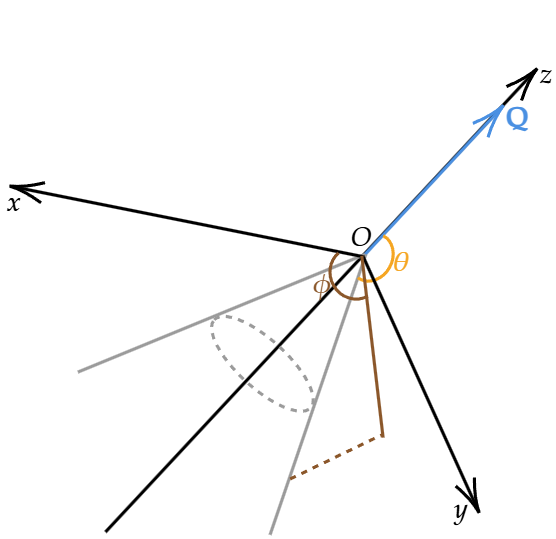
\includegraphics[width=6cm, height=6cm]{Content/Figure/magnetic_monopole.png}
    \end{figure}
        \end{column}
        \begin{column}{0.5\textwidth}
            \begin{itemize}
                \item \(\mathbf{Q}\cdot\hat{\phi}=mr^2\dot\theta=0\implies \theta=const\).
                \item \(\mathbf{Q}\cdot\hat{r}=Q\cos\theta=-kq_e q_m \implies \lvert \mathbf{Q}\rvert =const\).
                \item \(r(\phi)=\frac{Q\sin\theta}{mv\cos((\phi-\phi_0)\sin\theta)}\).
            \end{itemize}
            
        \end{column}
    \end{columns}
\end{frame}